\documentclass[border=5pt]{standalone}
\usepackage{tikz}
\usepackage{amsmath}
\usetikzlibrary{calc, positioning, arrows.meta, 3d}
\begin{document}
% Triangle with horizontal strips
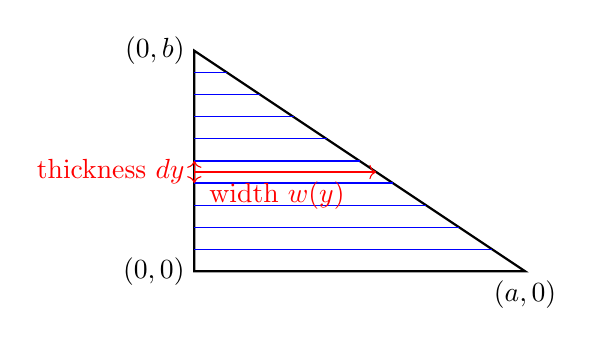
\begin{tikzpicture}[scale=1.4]
% Draw triangle divided into strips
\draw[thick] (0,0) -- (3,0) -- (0,2) -- cycle;
\node[left] at (0,0) {$(0,0)$};
\node[below] at (3,0) {$(a,0)$};
\node[left] at (0,2) {$(0,b)$};

% Draw horizontal strips
\foreach \y in {0.2,0.4,0.6,0.8,1.0,1.2,1.4,1.6,1.8} {
  \draw[thin, blue] (0,\y) -- ({3-1.5*\y},\y);
}

% Highlight one strip
\draw[red, ->] (0,0.9) -- (1.65,0.9);
\node[red, below] at (0.75,0.9) {width $w(y)$};
\draw[red, <->] (0,0.8) -- (0,1.0);
\node[red, left] at (0,0.9) {thickness $dy$};

\end{tikzpicture}

\vspace{1cm}

% General triangle decomposition
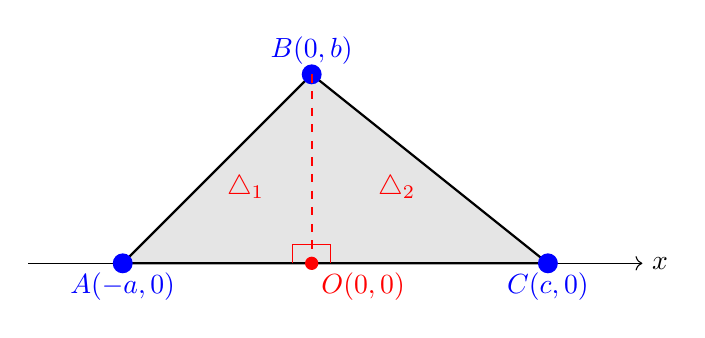
\begin{tikzpicture}[scale=1.2]
% Draw coordinate axes
\draw[->] (-3,0) -- (3.5,0) node[right] {$x$};


% Draw triangle
\draw[thick, fill=gray!20] (-2,0) -- (0,2) -- (2.5,0) -- cycle;
\fill[blue] (-2,0) circle (3pt) node[below] {$A(-a,0)$};
\fill[blue] (0,2) circle (3pt) node[above] {$B(0,b)$};
\fill[blue] (2.5,0) circle (3pt) node[below] {$C(c,0)$};

% Draw decomposition line
\draw[thick, red, dashed] (0,2) -- (0,0);
\fill[red] (0,0) circle (2pt) node[below right] {$O(0,0)$};

% Label the two right triangles
\node[red] at (-0.7,0.8) {$\triangle_1$};
\node[red] at (0.9,0.8) {$\triangle_2$};

% Mark right angles
\draw[red] (-0.2,0) -- (-0.2,0.2) -- (0,0.2);
\draw[red] (0.2,0) -- (0.2,0.2) -- (0,0.2);
\end{tikzpicture}
\end{document}
